\section{Results}

To build our observation model \eqref{eq:2gram_model}, we build simulated
worlds with randomly placed objects, generate LIDAR scans from these worlds, and
populate a lookup table of histograms.

Then, we generate a LIDAR scan from an unseen simulated world with multiple
objects. This is shown in \figref{fig:sim_world}.

We run our detector on this LIDAR data. Detections accumulated across all
orientations using the 1-gram model are shown in \figref{fig:star_1gram} and
\figref{fig:box_1gram}, and using the 2-gram model in \figref{fig:star_2gram}
and \figref{fig:box_2gram}.
%
\begin{figure}
  \centering
  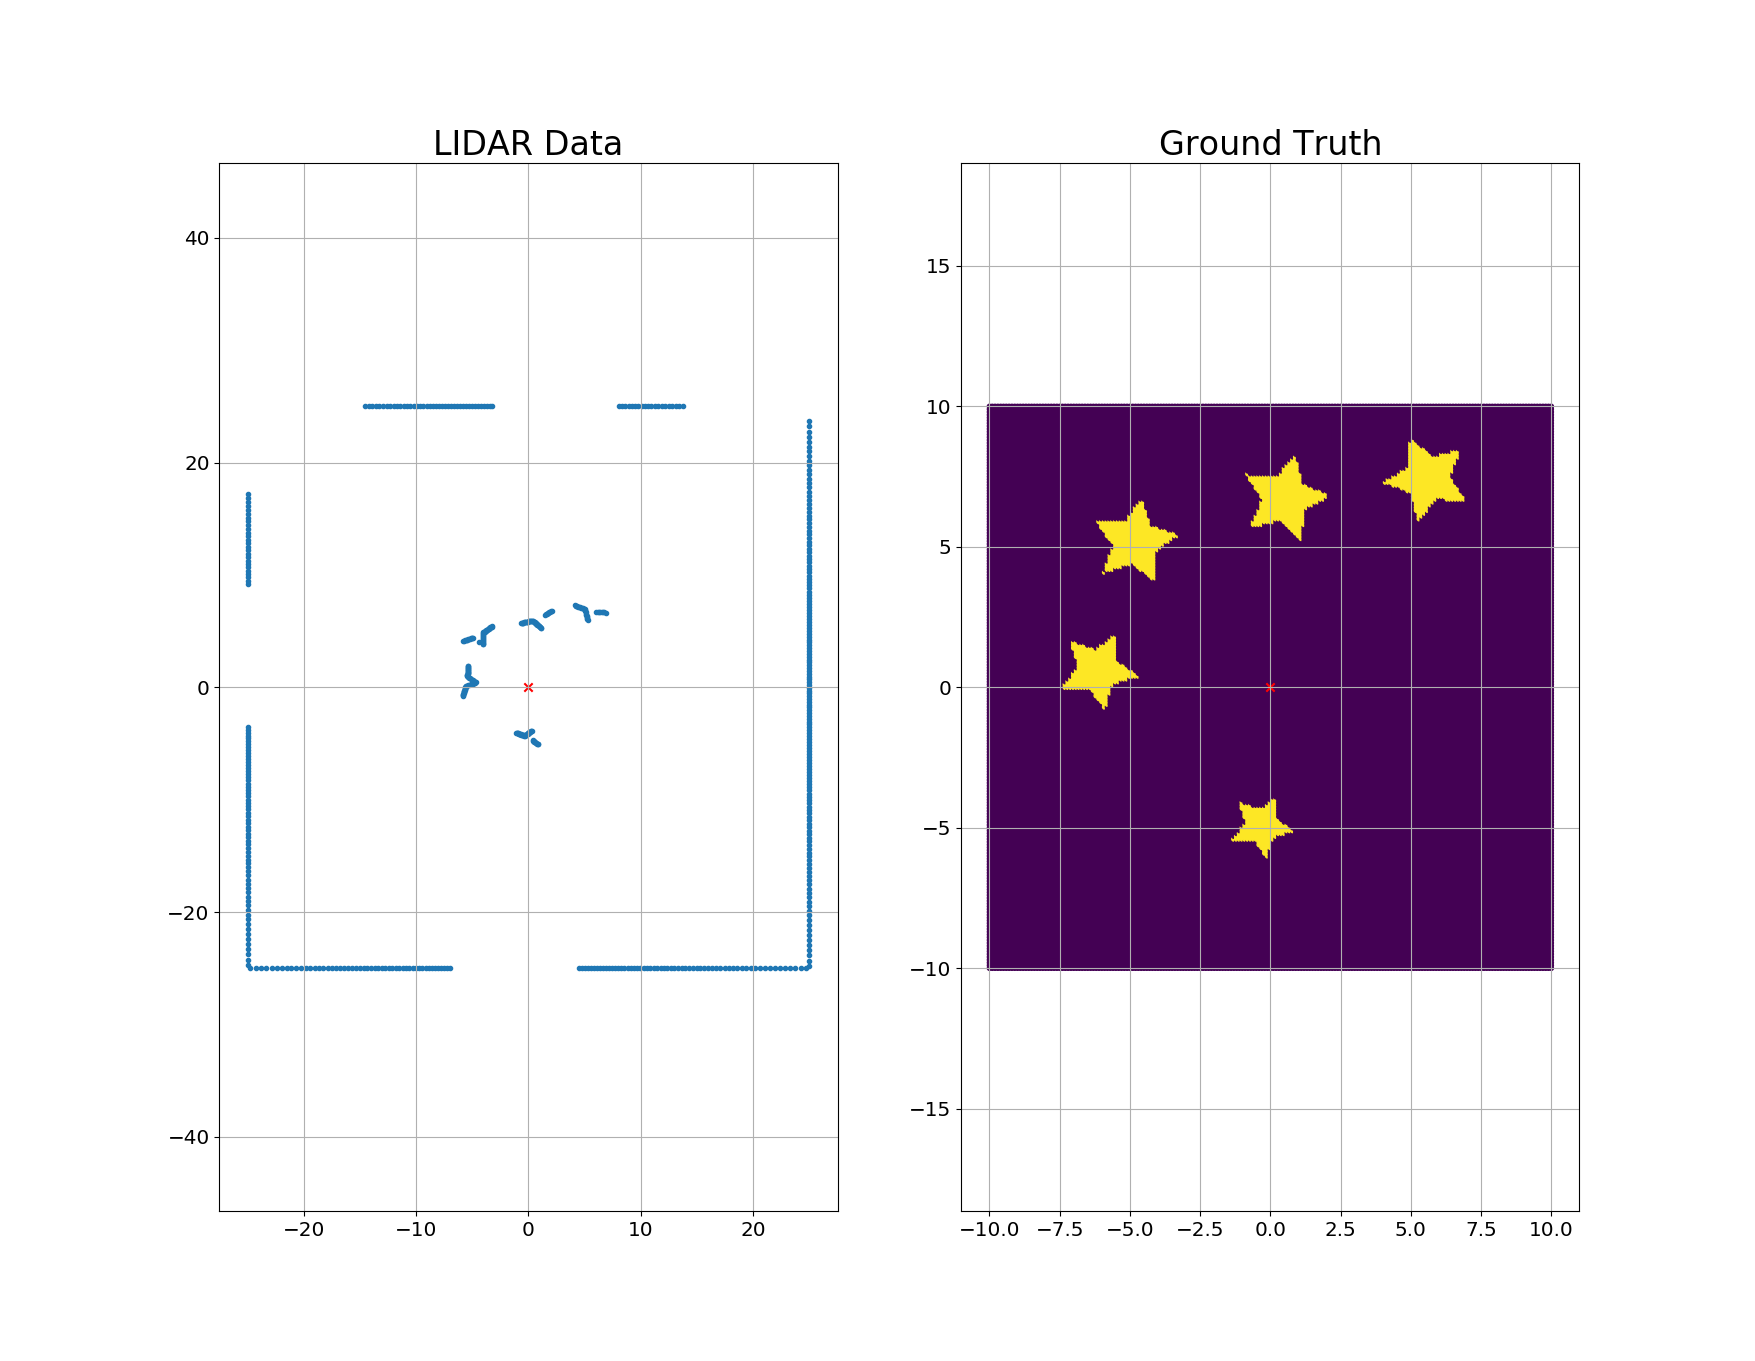
\includegraphics[width=\columnwidth]{figures/ground_truth.png}
  \caption{Simulation. On the left is the simular LIDAR scan of the environment.
    The right figure depicts the ground truth position of all objects in the
    scene.}
  \label{fig:sim_world}
\end{figure}
%
\begin{figure}
  \centering
  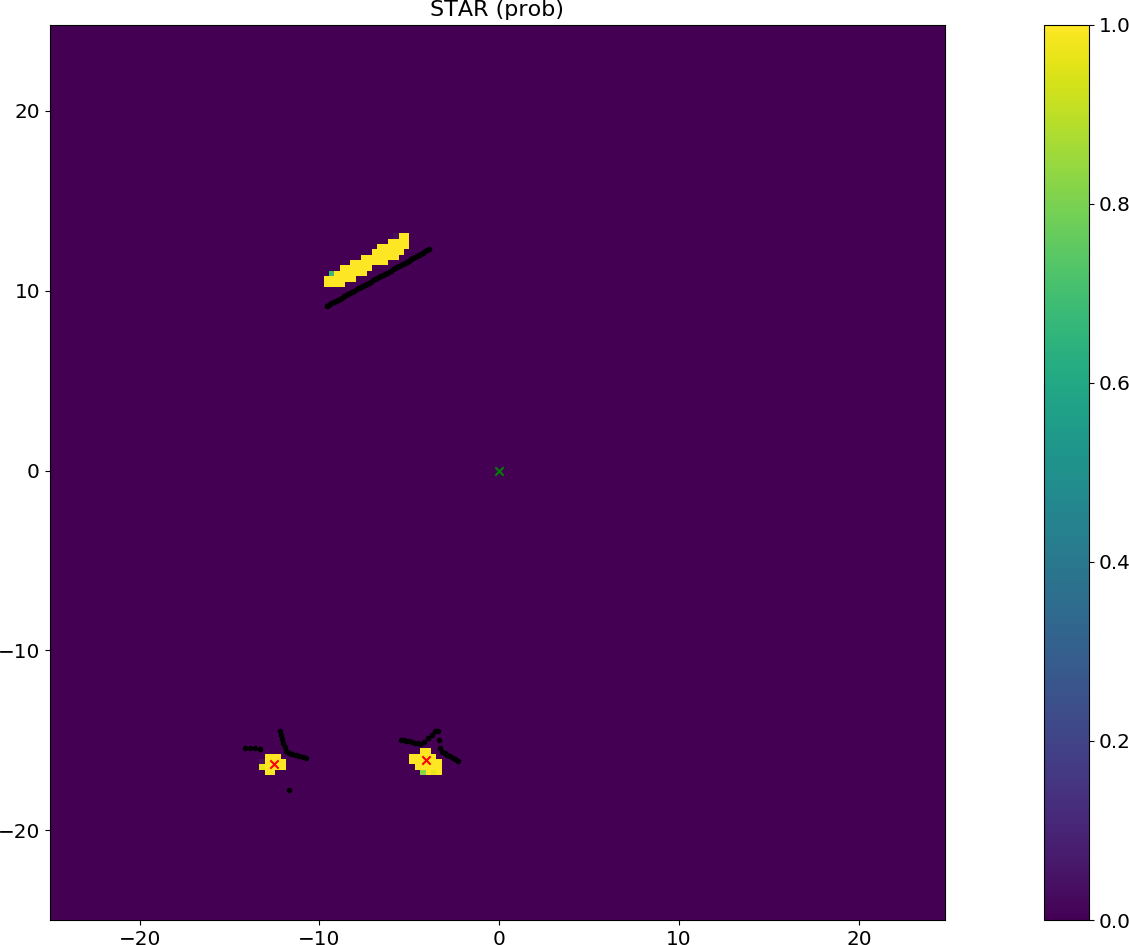
\includegraphics[width=\columnwidth]{figures/star_1gram.png}
  \caption{Star detections across all orientations for 1-gram model. Red x
    depicts ground truth.}
  \label{fig:star_1gram}
\end{figure}
%
\begin{figure}
  \centering
  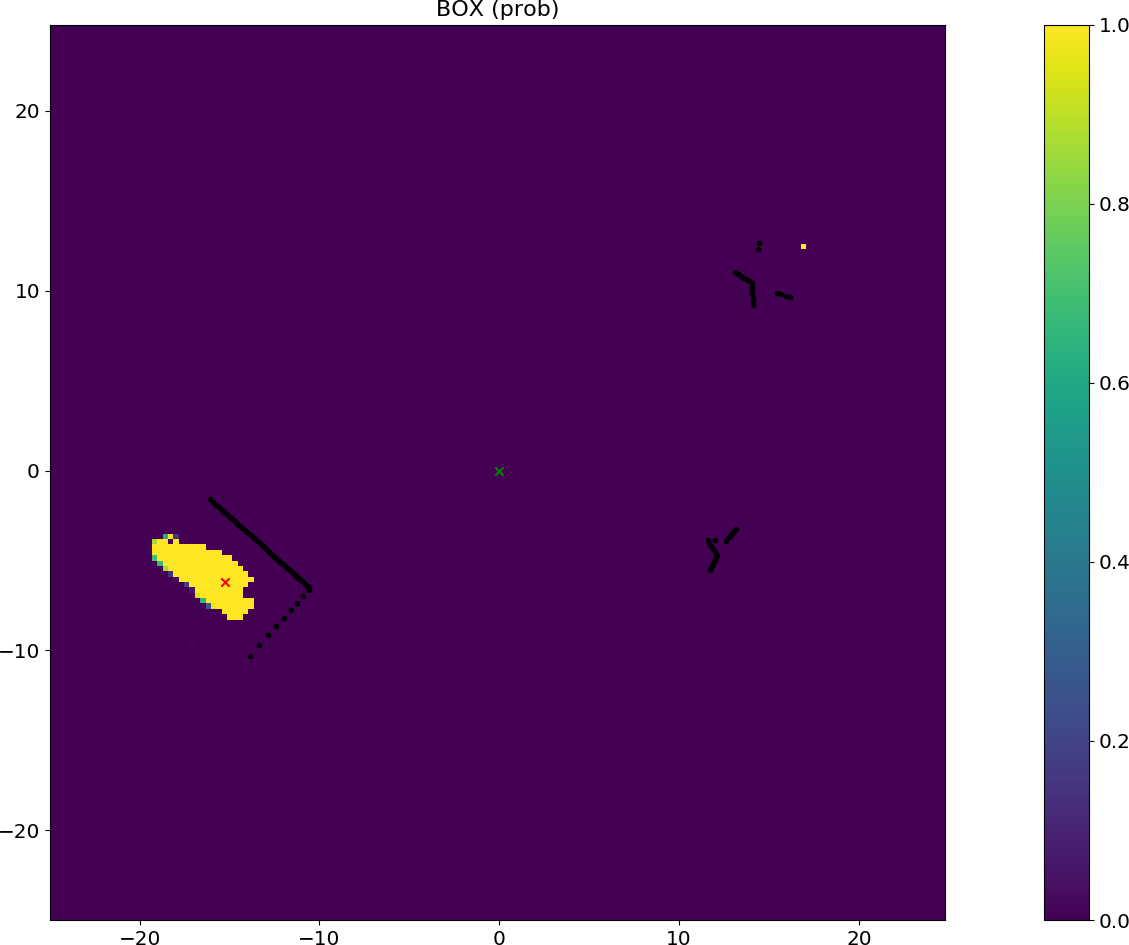
\includegraphics[width=\columnwidth]{figures/box_1gram.png}
  \caption{Box detections across all orientations for 1-gram model. Red x
    depicts ground truth.}
  \label{fig:box_1gram}
\end{figure}
%
\begin{figure}
  \centering
  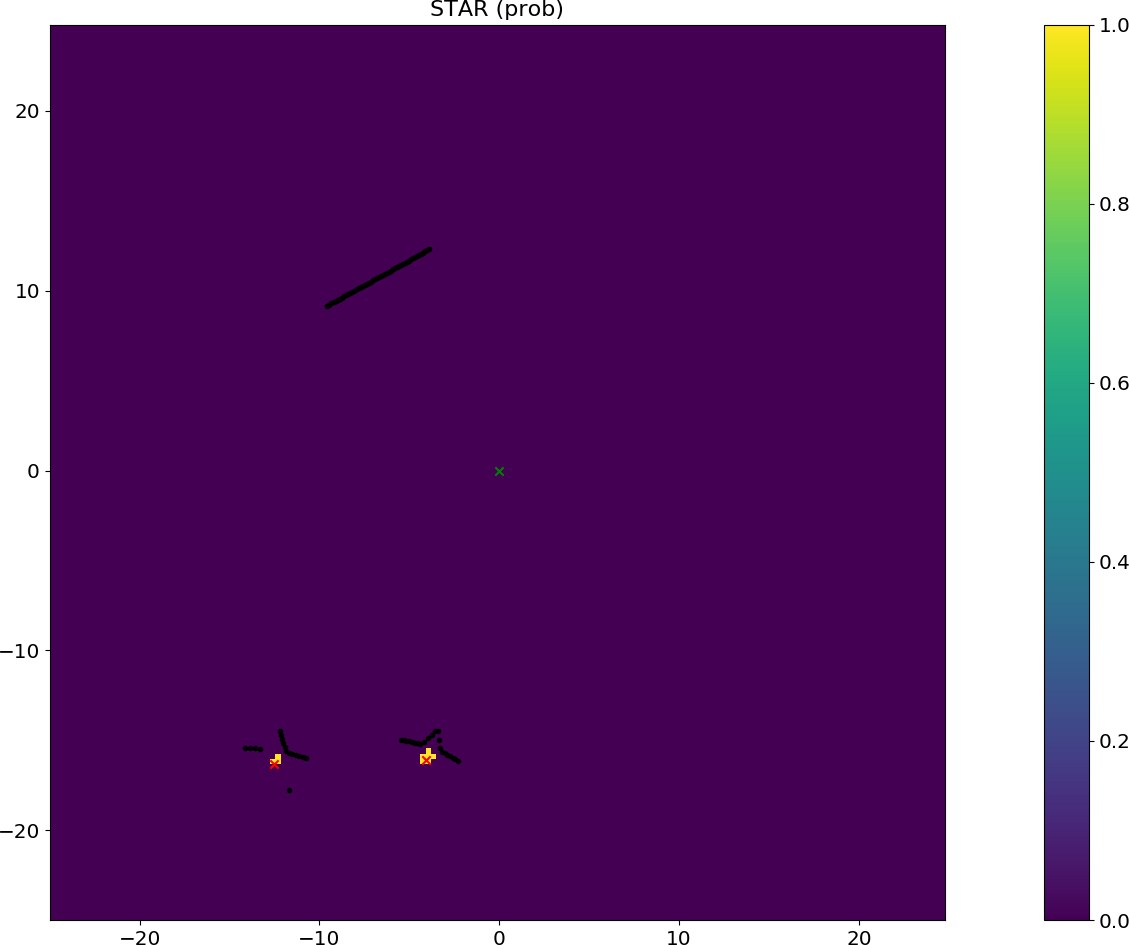
\includegraphics[width=\columnwidth]{figures/star_2gram.png}
  \caption{Star detections across all orientations for 2-gram model. Red x
    depicts ground truth.}
  \label{fig:star_2gram}
\end{figure}
%
\begin{figure}
  \centering
  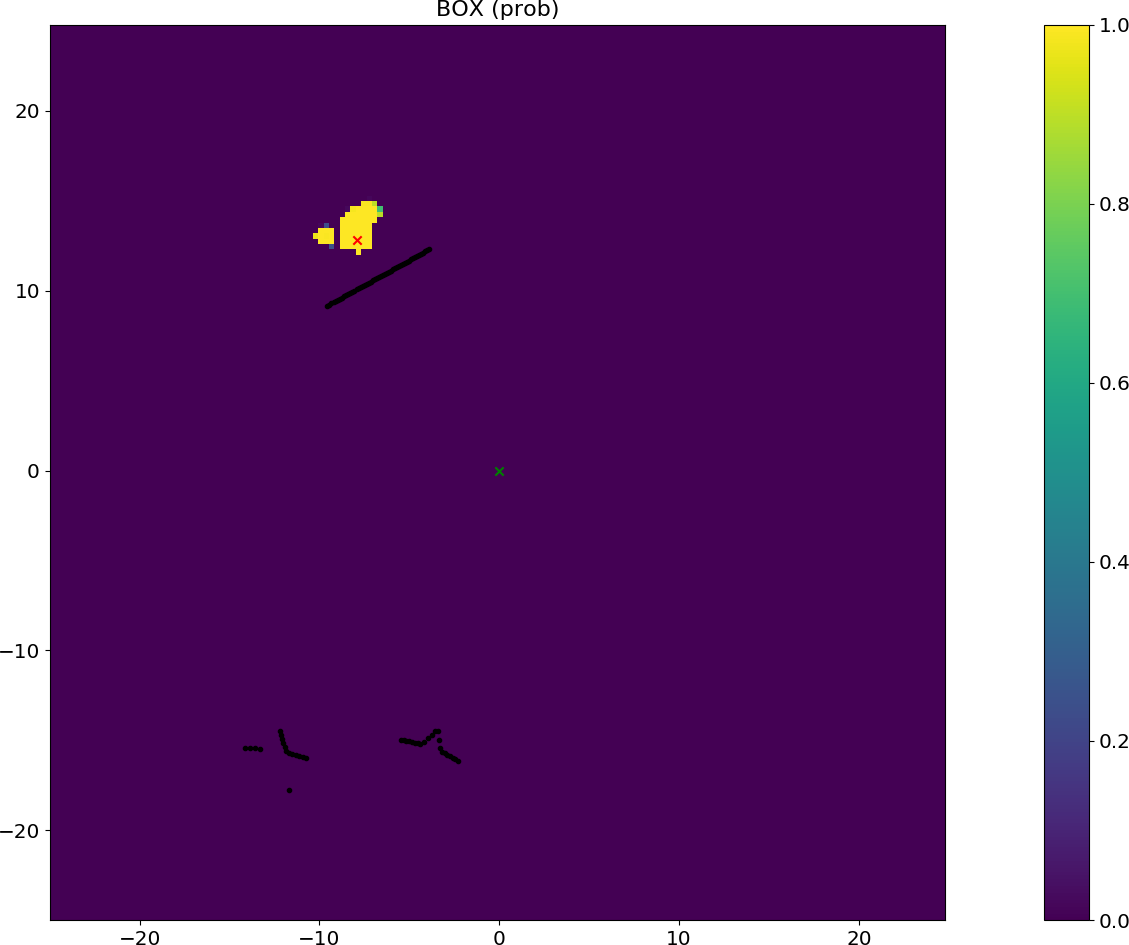
\includegraphics[width=\columnwidth]{figures/box_2gram.png}
  \caption{Box detections across all orientations for 2-gram model. Red x
    depicts ground truth.}
  \label{fig:box_2gram}
\end{figure}
